\documentclass[12pt,a4paper]{article}
\usepackage[utf8]{inputenc}
\usepackage[T1]{fontenc}
\usepackage[english]{babel}
\usepackage{parskip}
\usepackage{graphicx}
\usepackage{url}
\title{Checkers in Haskell}
\author{By: Daniel Jönsson, Madelene Alanenpää, Henrik Schulze }
\date{PKD 2017 - 2018}
\begin{document}
\maketitle
\newpage
\tableofcontents
\newpage

\section{Introduction}
After some discussions on what project to do we decided to make the game checkers in Haskell. Our programme lets two users play checkers in Haskell against each other. 

Checkers is an old game that can be played on a chessboard or on a bigger board. We decided to implement it on a chessboard with 8*8 squares. All the 12 pieces on each side of the board stand on the dark squares in the first 3 rows when the game starts. Figure \ref{fig:Checkers} is an example of the starting board for checkers.

Pieces always move diagonally so they will always stay on the black squares. A piece making a non-capturing move (not involving a jump) may move only one square in a forward direction. A piece making a capturing move (a jump) stands next to an opponent and leaps over one the opponent landing in a straight diagonal line on the other side. The jump can only be made if the square after the opponent is empty so only one piece may be captured in a single jump; however, multiple jumps with one piece should be made if that is possible during a single turn. The pieces can jump in both directions when capturing opponents.

When a piece is captured, it is removed from the board. If a player can make a capture, there is no option; the jump must be made. If captures are available for several pieces, the player is free to jump with whichever he or she prefers. When a piece reaches the furthest row from the player who controls that piece, it is crowned and becomes a king. A king has more freedom and can move several steps in a diagonal line if the line is free. When a king makes a jump, it can make it if the space behind the opponent is free even if the king is not standing next to that piece.

Our initial idea was to make the game in a few steps in Haskell. We would first make it so that two players could play against each other, then create a computer player that would be able to play in a simple way against a human and to implement gloss graphics for our game. It was a challenge to make the game so that two players could play against each other, so we decided only to stop after that since we didn’t have enough time to also implement a computer player. We also had some problems with implementing the gloss graphics in the game.


\begin{figure}

  \begin{center}
  	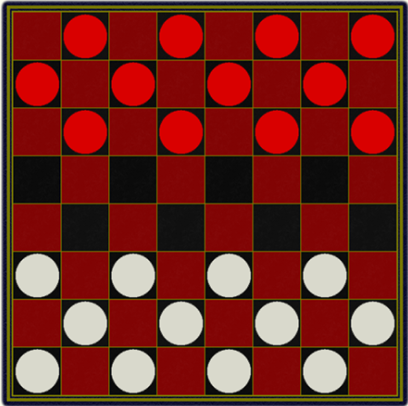
\includegraphics[width= 0.4\textwidth]{Startboarexample.PNG}
  \end{center}
	\caption{A Checkers start board.}
	\label{fig:Checkers}
\end{figure}
\begin{figure}
	\begin{center}
		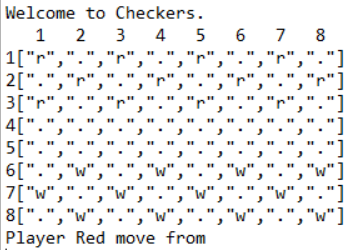
\includegraphics[width= 0.4\textwidth]{start.PNG}
	\end{center}
	\caption{A Checkers start board in Haskell.}
	\label{fig:Ch}
\end{figure}
\section{Summary}
So, what did we accomplish with our code? 

As mentioned in the introduction we did not manage to implement all the things that we had as goals such as creating a computer player and making the game available with Gloss graphics. However, we still feel satisfied with our work since we managed to make a functional game in Haskell so that it is possible for two human players to play the game.

In the start of the game it is only possible for the red player to make the first move and then the players take turns to move. The game follows the rules of checkers as described in the introduction with some small exceptions.

Pieces are put out diagonally on the first 3 lines of the board and from here they can only move diagonally. They can only move one step at a time unless they have the possibility to make one or several jumps. The pieces can’t jump outside the board and a piece will be removed once it has been jumped over. The player loses the game when he/she have no more pieces on the board. 

\section{Usage of Program}
In our game you will get a starting board see Figure \ref{fig:Ch} and from here you can start to play. To start you write a tuple with two numbers that represents from where you want to move and press enter. Then you write a new tuple for where you want to move, and press enter again. The first number in the tuple represents the row and the second represents the column.

Example below:
Player Red move from

(3,1)

Player Red move to

(4,2)

Player Red moves from  (3 , 1)  to  (4 , 2)

You will now get an updated board with the move applied and under the board it will say “Player white move from”. Like this the game will continue and if you make an unvalid move you will get a text that says "Invalid Move. You can only move your own pieces and move diagonally
Player Red move from"


\end{document}
